\section{Dataset Construction}
In this section, we introduce the construction of \textit{PsySym}, the first annotated multi-disease symptom identification dataset based on social media posts.

\subsection{Disease-Symptom Knowledge Graph}
\label{sec:kg}

Before data construction, we need to decide the annotation targets, i.e. which diseases and their corresponding symptoms to annotate. Considering our downstream application of MDD, we choose 7 diseases\footnote{We initially try to annotate the symptoms of all 9 diseases of SMHD, but we find it hard to plausible samples for \textit{Autism} and \textit{Schizophrenia}, and thus focus on the remaining 7.} that are used in the established SMHD dataset \citep{cohan2018smhd}: \textit{Depression, Anxiety, ADHD, Bipolar Disorder, OCD, PTSD, Eating Disorder}. We then find symptoms used in the diagnostic criterion of these diseases within DSM-5~\citep{american2013diagnostic}. However, the symptoms in DSM-5 are not represented as standard classes, but expressed in natural language with similar symptom having nuanced differences in different places. Therefore, we manually merge similar expressions of a symptom into one standardized class, and store the expressions as its detailed descriptions (also referred to as \textit{sub-symptoms}). After merging the symptoms, the diseases and the standardized symptoms constitute a bipartite Knowledge Graph (KG), where we can clearly see the shared symptoms of different diseases. We also supplement the KG with representative clinical questionnaires, where we also merge the symptoms mentioned in each question/item into the standard classes, and add links between the targeted disease and the measured symptoms if such edges are not found in DSM-5. The final knowledge graph (Figure \ref{fig:symp_kg}) has 45 nodes (7 diseases and 38 symptoms), and 162 edges. Symptoms like \textit{Depressed Mood} and \textit{Inattention} are shared by as many as 5 diseases, suggesting the potential of learning such shared features with multi-disease modeling. 

\begin{figure}[ht]
    \centering
    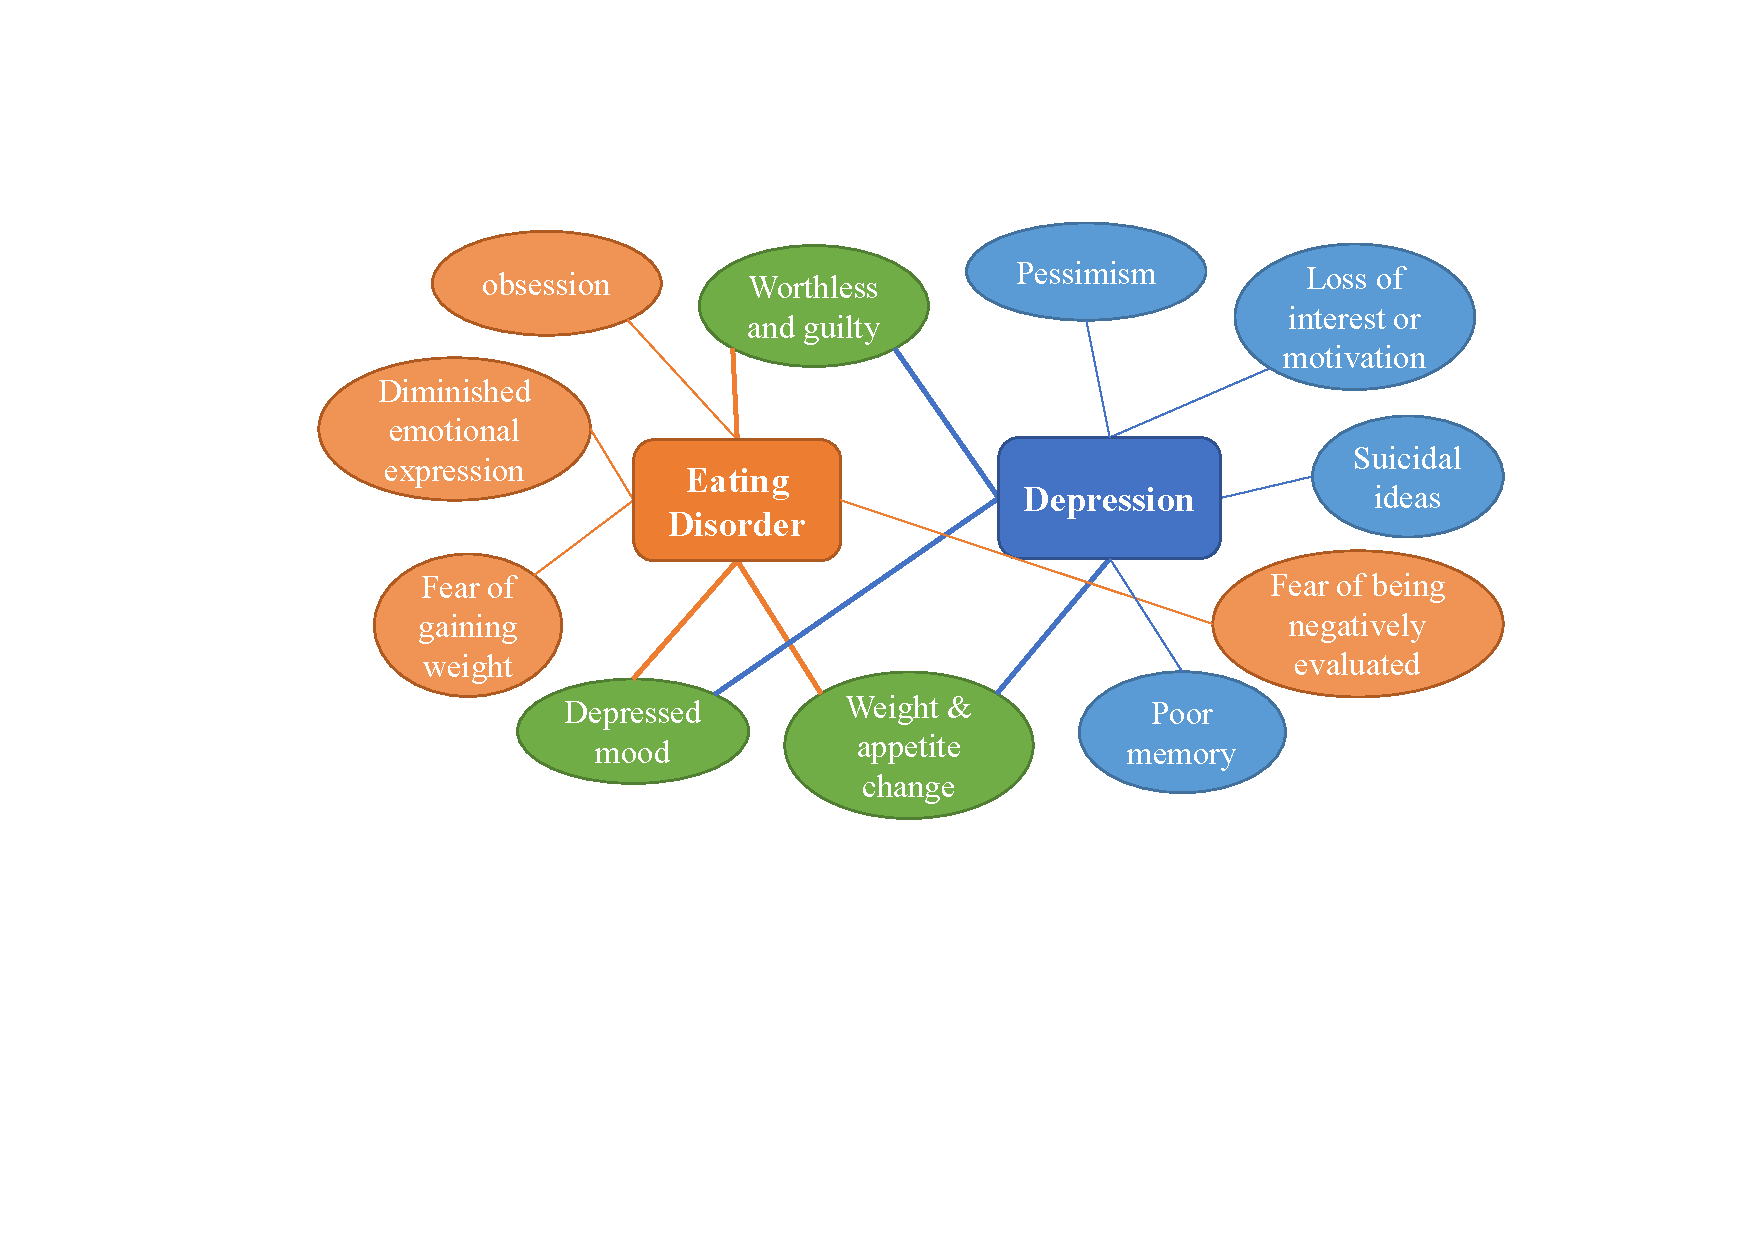
\includegraphics[width=1.0\columnwidth]{figures/symp_kg_v2.pdf}
    \caption{Illustration of the established disease-symptom knowledge graph. Only 2 diseases and their corresponding symptoms are shown for clarity. Many symptoms can be shared by multiple diseases, like the green nodes in the figure.}
    \label{fig:symp_kg}
\end{figure}

\subsection{Annotation Candidates Retrieval}
\label{sec:data_retrieval}

\begin{table*}[t]
    \small
    \centering
    \begin{tabular}{|l|l|l|}
    \hline
        Post & Symptom(s) & Status  \\ \hline
        Libido, pls come back! & Genitourinary (loss of libido) & True  \\ \hline
        I feel sad and motivationless. & Depressed; Loss of Interest or Motivation & True  \\ \hline
        I'm questioned if I'm manic. & Mood Shift & Uncertain  \\ \hline
    \end{tabular}
    \caption{Example annotations in PsySym. We can match the first post with a sub-symptom (loss of libido) of genitourinary system despite its figurative style. The second post has multiple labels. The symptom in third post is ambiguous, so we provide a distinct ``Uncertain'' label for its symptom status.}
    \label{tab:label_example}
\end{table*}

We then search for candidate posts to annotate the symptoms. We choose Reddit as our data source for its public availability and wide acceptance in previous literature \citep{losada2016test,cohan2018smhd,wolohan2018detecting}. Specifically, the candidate pool consists of all self-posts from 2005 to 2016 in the PushShift dataset \citep{baumgartner2020pushshift}, and all posts are split into sentences for later usage. 

The huge amount of posts necessitate a pre-step of selecting candidates that are likely to express certain symptoms for acceptable annotation efforts. First, we only select candidates from mental health related subreddits \citep{cohan2018smhd}, where more posts will be relevant. Moreover, we leverage embedding-based retrieval to further narrow down the range\footnote{We designed an algorithm to promote the balance of all symptoms classes. Details in Appendix \ref{apd:cand}.}. Specifically, we use Sentence-BERT \citep{reimers-2019-sentence-bert} to encode the post sentences and the symptom descriptions in the KG into embeddings. Then we will calculate the cosine similarity between them, and estimate a sentence's relevance to a symptom with its max similarity with all of the symptom's sub-symptoms. The rationale is that a symptom can have different manifestations expressed in its descriptions, and a sentence can be considered to convey that symptom if it resembles any one of them. However, since the original symptom descriptions in DSM-5 are expressed in a professional style and usually observed as a third party, they do not necessarily reflect 
the self-reporting nature of the content on social media. 
The descriptions collected from clinical questionnaires, however, can alleviate the problem, as they are designed to be easy to understand and fill in. To further tackle the mismatching that cannot be solved even with the questionnaires, we also directly collected some typical Reddit posts about a symptom for the similarity calculation in place of the official descriptions. We will show in \S\ref{sec:exp_retrieve} that our final method can lead to better precision and recall for the retrieved candidates, compared with the keyword/pattern matching methods commonly used in previous works \citep{mowery2017understanding,yadav2020identifying}.

\subsection{Annotation Design}
\label{sec:data_annotation}

Annotations for symptom identification usually involve the binary decisions if a symptom can be identified from the sentence. Such decision can sometimes be tricky when a symptom is mentioned in a sentence, but is not actually present. For example, ``I don't have panic attack.'' implies a \textit{negation} of the symptom, and ``Is it panic attack?'' expresses the \textit{uncertainty} about the symptom. Although most previous works like \citet{nguyen2022improving} treat such cases as negative samples, we think that they are different from the other negatives like sentences totally irrelevant to any symptoms or only about other symptoms. Distinguishing between them may enable a more informative analysis and benefit downstream applications. Therefore, we decided to divide the annotation into two tasks: \textbf{relevance judgment} and \textbf{status inference}, as are exemplified in Table \ref{tab:label_example} and Table \ref{tab:more_label_example}. For relevance judgment, the annotator needs to judge whether the sentence is relevant to the given symptoms. Note that the symptoms can be described in figurative language instead of standard patterns, and they can be negated or uncertain. For status inference, the annotator needs to decide, if the relevant symptom(s) are indeed present. We denote positive/negative status as `True'/`Uncertain'.

Before crowdsourcing annotation, we first conducted preliminary annotations ourselves. We found it hard to annotate all 38 symptoms among the candidates from all mental health subreddits. The relatively large number of classes, and the nuanced differences and similarities between them can pose heavy cognitive burden to the annotators. Therefore, we decided to separate the annotation job queues by disease. In each queue, the annotators only need to read the posts from the subreddits of that disease, and the symptoms are restricted to only the typical symptoms of the disease according to our KG. Although this transformation can potentially affect the recall of atypical symptoms, we find it significantly improve the annotation efficiency and agreement in our preliminary tests. 

We then invite volunteers for the annotation tasks, who are all well-educated and also include professional psychiatrists. To ensure the data quality, each sentence is annotated by 3 participants, and we also utilize a series of quality control protocols. The annotation proceeds as follows: 
\begin{enumerate}
    \item Training Session: We train the annotators about the annotation rules and also demonstrate some example annotations by ourselves through video meetings.
    \item Screening Tests: We collect test questions from samples on which the authors have consensus in preliminary annotations. The invited volunteers need to first annotate on these questions and achieve certain score to be eligible for further annotation. They can take the test for several times, and we require them to read the reason for our decision after the test for their better alignment with our requirements.
    \item Annotation: Those who passed the screening tests can proceed for further annotation. During annotation, they can always discuss with us about any questions encountered.
    \item Sampling Inspection: At intervals, we will sample 10\% of the completed annotations from an annotator for checking. We will correct any annotations we find inappropriate, and give a score according to the number of corrections. If the score is below certain threshold, all annotations in the checking batch will be rejected for re-labeling.
\end{enumerate}

Finally, we recruited 31 volunteers contributed valid annotations for 8,554 sentences. The average Fleiss's $\kappa$ for the relevance judgement of all 38 symptoms is 0.7708, and the $\kappa$ of status inference is 0.2518. Among all symptoms, \textit{Anxious Mood} has the most labels (1764), while \textit{Avoid Stimuli} has the least (78). For status inference, the `Uncertain' annotation constitutes 13.75\% for all annotations. More details are provided in Appendix \ref{apd:stats}.

\subsection{Labels and Data Splits}

To merge the multiple annotations into a single gold label for each sentence, we consider a symptom to be relevant to a sentence as any one of the annotation is positive, and we use the portion of \textit{uncertain} annotations as the label for status inference (more discussion in \S \ref{sec:model_status}). We split the dataset into training/validation/testing set by 5:1:4 to preserve enough samples for all classes in the test set for a stable evaluation. 

To allow models to accurately identify symptoms from all posts of social media, where the majority of them are not related to any mental disease symptoms, we also collect such posts (referred to as \textit{control posts}) for PsySym from the same candidate pool. We randomly sample posts whose author doesn't have any post or comment in mental health related subreddits, and further remove posts that contain any mental health related terms provided by \citet{cohan2018smhd}. Finally, we randomly sample sentences from the remaining posts, resulting in 83,779 sentences, distributed into training/validation/testing set by 5:1:4.

\subsection{Disease Detection Dataset}
\label{sec:data_disease}

To demonstrate the helpfulness of PsySym for the downstream task of MDD, we also construct a dataset by reimplementing the data collection method of SMHD \citep{cohan2018smhd}. We find diagnosed users by the pattern-matching of two components: one that indicates a self-reported diagnosis (e.g. ``diagnosed with'), and another that maps relevant keywords to the 9 mental diseases (e.g. ``panic disorder'' to \textit{Anxiety}). A user is labeled with a disease if one of its keywords occurs within 40 characters of the diagnosis pattern. Control users are randomly sampled from those who never posted or commented in mental health related subreddits. Similar to SMHD, we eliminate the diagnostic posts from the dataset to prevent the direct leakage of label, but we don't remove other mental health related posts to allow the extraction of symptom-related features. The final dataset consists of 5,624 diagnosed users and 20,981 control users with average number of posts per user being 102.5 and 119.4, respectively. We provide the distribution of each disease in Appendix \ref{apd:stats}. 
